\documentclass[../main]{subfiles}
\begin{document}

\section{Environment Configuration}
Configuring your environment can be quite frustrating at times and can eat away a lot of time. For that reason,
here are some detailed instructions for getting you set up quickly. Moreover, it is also helpful to know how to configure a
modelling project. An unorganised project saps away productivity so I also detail here one way of organising your
project specifically for modelling with PyCoTools, COPASI and tellurium.

It would be helpful the configuration steps below were done prior to the workshop
as then we can focus on modelling issues, rather than configuration issues.

\subsection{Python}
Python is a program written in C. There are many `distributions' of Python, which essentially just means
different people have compiled it and packaged it in slightly different ways.

My favourite distribution of Python is \href{https://docs.conda.io/en/latest/miniconda.html}{Miniconda}. Miniconda
and Anaconda are essentially the same, but Anaconda comes with a whole bunch of additional Python packages. These
can be useful, but it is quicker to just use Miniconda.

\begin{Task}[label=InstallMiniconda]{Install Miniconda}
Google Miniconda and follow the instructions to install Miniconda.
\end{Task}

\warning{Make sure the command \bash{conda} works from terminal or cmd. If it doesn't, then you
need to add the Miniconda bin directory to your path environment variable.}

Anaconda and Miniconda (or just Conda) allow you to create isolated Python environments
and switch between them easily. Think of each \bash{conda} environment as a box that is
kept separate from the other Python `boxes'. While the full documentation can be
found \href{https://docs.conda.io/projects/conda/en/latest/user-guide/tasks/manage-environments.html}{here},
the commands to create a \bash{conda} environment are quite simple.

\begin{minted}{bash}
$ conda create --name py36 python=3.6
\end{minted}

Will create a conda environment.

\begin{minted}{bash}
$ conda activate py36
\end{minted}

will switch to the environment

and

\begin{minted}{bash}
$ pip install pycotools3 tellurium
\end{minted}

will install \bash{pycotools3} and \bash{tellurium} with all their dependencies.

\warning{Neither \bash{pycotools3} nor \bash{tellurium} work on Python 3.7 or 3.8. This is because of
a broken dependency. The issue is in the process of being solved (apparently).}

\subsection{COPASI}

\begin{Task}{Install COPASI}
Install Copasi and configure the environment variables if you need to
(\href{https://pycotools3.readthedocs.io/en/latest/#troubleshooting}{instructions}). You should be able to
run \bash{CopasiUI} from the terminal.
\end{Task}

\subsection{PyCharm}
PyCharm is a significantly better IDE than many of the alternatives. It does a lot for you. You can also
get a free Licence for the Pro edition with your university email address. Learning how to use
PyCharm is useful for many reasons, one of which is that if and when you migrate to other programming
languages, JetBrains will have an IDE for you tailered to that language. Since all the IDEs are
very similar, you only have to learn to use one and the rest fall in place.

\begin{Task}{Install PyCharm}
Install PyCharm. I prefer to install the JetBrains toolbox and install the IDE from there.
\end{Task}
\begin{Task}{Install CellDesigner}
Install Cell Designer
\end{Task}
\begin{Task}{Install Github}
Install git and make a free GitHub account.
\end{Task}

\subsection{Configuring a Project}
With a small amount of effort, we can build an organised modelling project which will
dramatically enhanced productivity down the line when you need to extend the model and make changes.
We will be creating a project which contains a single Python package that itself has two subpackages
(see Figure \ref{fig:config:example_project}). We will also turn this project into a GitHub repository.
\begin{Task}{Python pacakges and modules}
If you are not familiar with the concept of Python packages, subpackages and modules, now might be a
good time to do a quick google to get a broad understanding  (no need to go overboard). This will
help you understand why the project is configured the way it is.
\end{Task}

\begin{Task}{Downloading the example project}
Since some aspects of configuring our project may initially be a bit confusing, clone, fork or
download the \href{https://github.com/CiaranWelsh/ExampleProject}{example project}.
This project contains a skeleton that you can use as a template.
The quickest way would be for go the link and press the \bash{fork} button. This will make a copy in your
own GitHub. Then go into the settings section of the respository on your own GitHub and
change the name to whatever you like. Now, clone your own repository
using \bash{git clone https://github.com/<your name>/<your project name>}.

\note{If you want to configure this yourself instead, you can omit this step and follow the instructions
below. If you download it, it's still a good idea to understand the prroject structure, by reading below. }.
\end{Task}

\begin{Task}{Create a Project}
We will be using a project structure that looks like that shown in Figure \ref{fig:config:example_project}.
If you haven't already downloaded the example project, create this structure somewhere in your file system.
In PyCharm, create a new project. Then navigate to the root of the tree you have just created (or downloaded)
and hit open.
\end{Task}

\begin{figure}[h]
\centering
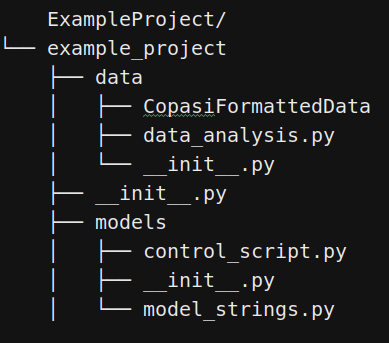
\includegraphics[width=0.4\linewidth]{EnvConfig/assets/example_project_config}
\caption{Directory tree for organised modelling project}
\label{fig:config:example_project}
\end{figure}

A package in Python is marked by the special file called \bash{__init__.py}. Even if it is a blank file,
the presence of this file in a directory marks it as a Python package. Whenever a package is imported, the
\bash{__init__.py} (for initialisation) is automatically executed. This makes it a convenient place to store
some variables that can be used anywhere throughout the project.

\begin{Task}{Configure Python Interpreter in PyCharm and Running Code}
We have created a Conda environment called \bash{py36}. Now we need to tell PyCharm to use this environment. At first,
PyCharm can feel unintuitive, but stick with it and it will enhance your productivity (trust me).

\begin{itemize}
\item Open the settings in PyCharm from the file menu
\item Select \bash{Project: <project name>} from the left, then project interpreter
\item We want to select the Python3.6 conda environment called \bash{py36}. If this is already in the dropdown
at the top of the screen, select it, press okay and then you're done. If not, continue.
\item Click on the gears icon, top right and press \bash{add} to tell PyCharm about a new Python interpreter.
\item Click on \bash{existing environment} and check the box that says \bash{make available to other environments}
\item Click the three dots to open up a file system and nagivate to the Python executable that you want to use.
\item On linux (or Mac) you can open a terminal, switch to your \bash{py36} environment using \bash{$ conda activate py36}
and type \bash{$ which python} to locate the Python executable. Copy and paste this into the box in PyCharm
and okay everything.
\item On Windows, you can do the same thing by opening a \bash{cmd} prompt or \bash{PowerShell}, switching to your
\bash{py36} environment using \bash{conda activate py36} then using the command \bash{> where python}. Copy and paste
the location of the Python executable into the box in PyCharm and then okay everything.
\item Now that you have configured PyCharm, you can create any Python script, right click somewhere and
press \bash{Run <script_name}, to run some Python code.
\end{itemize}

\end{Task}

Here is some information describing the components of the project.

\begin{itemize}
\item The main \bash{__init__.py} file (\bash{ExampleProject/example_project/__init__.py}) holds variables that
are used throughout the project. By keeping them in one place we never loose or forget about these
variables and we don't get conflicts resulting from duplicates. Examples of what variables we
will be defining in here include path names and flags for modifying the behaviour of the
program.
\begin{itemize}
\item \note{The other two \bash{__init__.py} files will be empty. This is only necessary to make your Python
modules importable.}
\end{itemize}
\item The \bash{model} package holds everything regarding your model such as the code for building and simulating a model
\item The \bash{model_strings.py} file functions as a storage module to keep model strings isolated from the execution code
\item The \bash{control_script.py} holds all code regarding actually loading and running simulations. It responds
to the variables defined in \bash{__init__.py} to modify what we actually want to do. For example, you could have
a variable called \bash{OPEN_WITH_COPASI} or \bash{CONFIGURE_PARAMETER_ESTIMATION}.
\item The \bash{data} module holds everything regarding experimental data, such as raw data
files and data analysis scripts.
\item The \bash{data_analysis.py} script does anything data
related (normalisation, plotting or automatically formatting for COPASI). For now, this will be empty but it will likely
be needed in the future.
\item The `CopasiFormattedData` folder holds all experimental data that is formatted for COPASI.
I usually do this programatically to save time in the long run but it can also be done in excel.
\end{itemize}

If you are not using the example project (which is already configured), a few pieces of code should
be added to this project before we begin modelling.

Firstly, if we want to import code from a Python module in your project (such as \bash{data_analysis.py},
\bash{__init__.py} or \bash{model_strings.py}) to where we want to use the code (\bash{control_script.py})
then we have to tell Python where the project is. To do this we point Python towards the directory containing
your package (i.e. the \bash{example_project} folder). Python has a special variable called the
PYTHONPATH variable that exists exactly for this reason. The template code below in \bash{control_script.py}
does this using the \python{site.addsitedir} function. If this doesn't make much sense to you,
don't get hung-up on it. This is a Python issue that a better understanding of the Python
module hierarchy will sort out. For now, just insert the code shown  below and forget about it.

\note{PyCharm has options in \bash{run configuration} for adding your project directories to the \bash{PYTHON_PATH}
variable. These are usually set to True by default, so if you use PyCharm, you actually don't need this step.
However, if the code is ported to another IDE (such as Spyder) you may run into problems}

\begin{Task}{Configure the control script}
\begin{minted}{python}
# ExampleProject/example_project/models/control_script.py
import os
import site
# Add path to sources root to Python's PATH variable
site.addsitedir(os.path.dirname(os.path.dirname(os.path.abspath(''))))
# note: Pycharm already does this for you.
# But doesn't hurt to add it here anyway

# Get the model string by importing it from your models_strings module
from example_project.models.model_strings import model_string

# imports all the global variables (notice that we
# can print out the WORKING_DIRECTORY variable)
from example_project import *


# Any functions or classes you write will go here

if __name__ == '__main__':

# Any code that uses the functions or classes your have created above,
# will go here. We will be using flags defined in our __init__.py
# to modify the behaviour of this script. Since the Flags are boolean,
# we just us a simple if statement for each of them

if PRINT_WORKING_DIRECTORY:
    # prints /home/ncw135/Documents/ExampleProject/example_project
    print(WORKING_DIRECTORY)
\end{minted}
\end{Task}

\begin{Task}{Configure the the projects \bash{__init__.py}}
\begin{minted}{python}
# ExampleProject/example_project/__init__.py
import os, glob
# Global variables are always in caps, to distinguish them from local variables.
WORKING_DIRECTORY = os.path.dirname(__file__)
DATA_DIR = os.path.join(WORKING_DIRECTORY, 'data')
COPASI_FORMATTED_DATA_DIR = os.path.join(DATA_DIR, 'CopasiFormattedData')

# Flags that change the behaviour of the control_script

# flag to demonstrate the principle of flags
PRINT_WORKING_DIRECTORY = True

\end{minted}
\end{Task}

We can now import the various parts of the project
within the \bash{control\_script} and begin modelling.

\note{If something isn't working and you've spent too much time trying to fix,
you can clone or fork my example \href{https://github.com/CiaranWelsh/ExampleProject}{project} from Github}.

\subsection{GitHub}
Git and GitHub are one of your most important tools. When used correctly you can version your code,
that if you make some changes that made your model worse, you can always revert to an
earlier verison. Moreover, it makes sharing code, models, simulations and working together much, much easier.

\begin{Task}{Create a GitHub Repository}
Sign up for a GitHub account if you do not already have one. Turn your version of this boiler plate
project into a GitHub repository. One set of instructions can be found
\href{https://help.github.com/en/github/getting-started-with-github/create-a-repo}{here}.
\note{This task can be safely omitted and not impact the rest of the project. However
I recommend that you at least figure out the basics. }
\end{Task}

\end{document}